\maketitle
\setcounter{page}{1}
\tableofcontents
\newpage
\pagenumbering{arabic}
\section{Theorie}
Licht als elektromagnetische Welle breitet sich als ebene Welle nach der Gleichung
\begin{equation}
  \vec{E}(x, t) = \vec{E}_0 \, \symup{cos}(kx-\omega t - \delta)
  \label{eqn:2}
\end{equation}
aus. Dabei ist $E$ die elektrische Feldstärke, $k$ die Wellenzahl, $\omega$ die Kreisfrequenz und $\delta$ der Phasenwinkel.
Wenn für das Licht die Maxwellschen Gleichungen und das Prinzip der linearen Superposition
gilt, dann lässt sich die Überlagerung mehrerer Lichtwellen einfach aus der vektoriellen Addition
der Wellengleichungen bestimmen. Da es aber aufgrund der hohen Lichtfrequenz nicht möglich ist,
diese experimentell zu bestimmen, wird stattdessen die Intensität betrachtet, die sich über
die Beziehung
\begin{equation*}
    I \propto |\vec{E}|^2
\end{equation*}
aus der elektrischen Feldstärke ergibt. Mit einigen Vereinfachungen folgt somit für die Intensität
überlagerter Lichwellen
\begin{equation}
  I = 2 \cdot \symup{const} \, \vec{E}_0^2 \, \symup{cos}(\delta_2 - \delta_1) \, .
  \label{eqn:1}
\end{equation}
Somit ist die Intensität der überlagerten Welle abhängig von der Differenz der Phasenwinkel.
Auch eine komplette Auslöschung ist möglich, falls die Differenz ungerade Vielfache von
$\pi$ ergibt.

Da die Phasenwinkel bei konventionellen Lichtquellen statistische Funktionen der Zeit sind,
fällt der Interferenzterm mei der Mittelung über einen großen Zeitraum weg. Deshalb
ist es wichtig, sogenanntes kohärentes Licht zu benutzen. Diese Art des Lichts zeichnet sich
dadurch aus, dass $k$, $\omega$ und $\delta$ in \eqref{eqn:2} konstant sind. Dies wird durch
die Verwendung von Lasern realisiert. Diese sind zwar nicht im Unendlichen kohärent, doch für die
im Experiment verwendeteten Längenskalen ausreichend. Damit sind alle Vorraussetzungen für
die Interferenzfähigkeit des Lichtes vorhanden.  \\
\\
Der prinzipielle Aufbau das Michelson-Interferometers ist in Abbildung \ref{fig:1} dargestellt. Dabei
ist L die Lichtquelle, $\symup{S}_1$ und $\symup{S}_2$ Spiegel, P ein semipermeabler Spiegel
und D ein Photodetektor.
\begin{figure}[h]
  \centering
  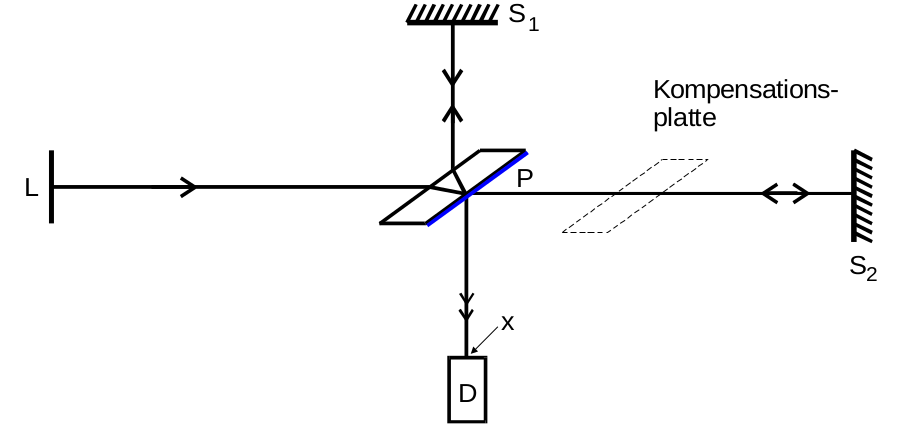
\includegraphics[scale=0.3]{michelson.png}
  \caption{Prinzipieller Aufbau des Michelson-Interferometers.}
  \label{fig:1}
\end{figure}
Um Interferenzeffekte untersuchen zu können, wird der Lichtstrahl
am semipermeablen Spiegel P in zwei Teilstrahlen aufgespalten. Einer setzt seinen Weg ohne Richtungsänderung fort,
der andere senkrecht zur Einfallsrichtung. Nachdem beide Strahlen an $\symup{S}_1$ bzw. $\symup{S}_2$
gespiegelt worden sind, treffen sie erneut auf P und werden erneut wie oben beschrieben aufgespalten. Damit die beiden Teilstrahlen
kohärent sind, werden die Abstände $\overline{\symup{S}_1 \symup P}$ und $\overline{\symup{S}_2 \symup P}$
annähernd gleich gewählt und eine Kompensationsplatte mit gleichem Brechungsindex und gleicher Dicke wie P
zwischen P und $\symup{S}_2$ gebracht, da im Gegensatz zu dem von $\symup{S}_1$ kommenden Strahl der
von $\symup{S}_2$ kommende Strahl P nur einmal statt dreimal durchläuft. Sind diese Vorraussetzungen
erfüllt, dann ensteht ein Gangunterschied von $\lambda / 2$ zwischen den beiden Teilstrahlen.
Somit löschen sich die beiden Strahlen aus und der Photodetektor D erfasst an der Stelle x
einen dunklen Fleck. Wird einer der beiden Spiegel um ein Stück d verschoben, ergibt sich statt
$\lambda / 2$ ein Wegunterschied von $2 \cdot d$ und die am Photodetektor D erfasste Intensität
ändert sich. Wenn man d kontinuierlich ändert, oszilliert die Intensität zwischen 0 (Auslöschung)
und dem Maximalwert. Somit lässt sich der Aufbau zur Wellenlängenbestimmung nutzen und es ergibt sich
\begin{equation}
  \symup{\Delta} d = z \frac{\lambda}{2} \ \ \text{bzw.} \ \ \lambda = \frac{2 \symup{\Delta} d}{z} \, .
  \label{eq:1}
\end{equation}
Dabei ist $z$ die Anzahl der Intensitätsmaxima. \\
\\
Eine andere Nutzungsweise des Michelson-Interferometers ist die Bestimmung von Brechungsindizes.
Der Aufbau ist in Abbildung \ref{fig:2} dargestellt.
\begin{figure}[h]
  \centering
  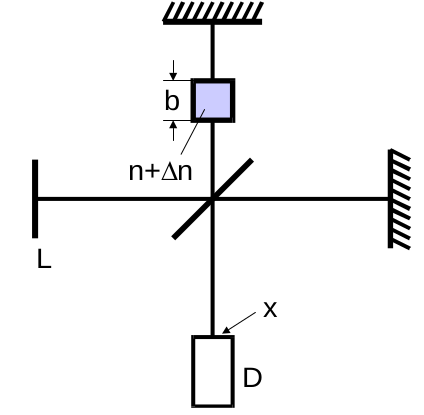
\includegraphics[scale=0.35]{n.png}
  \caption{Aufbau des Michelson-Interferometers zur Bestimmung von Brechungsindizes.}
  \label{fig:2}
\end{figure}
Das Medium der Dicke $b$ soll den Brechungsindex
$n + \symup{\Delta} n$ besitzen, an allen anderen Orten im Versuchsaufbau sei er $n$. Wird $\symup{\Delta} n$
langsam erhöht, erscheinen weder wechselnde Intensitäten an der Stelle x. Dabei entspricht $b \cdot \symup{\Delta} n $
gerade $\symup{\Delta} d$ aus \eqref{eq:1} und es ergibt sich
\begin{equation}
  b \cdot \symup{\Delta}n = \frac{z \lambda}{2} \, .
  \label{eq:2}
\end{equation}
Um aus $\symup{\Delta} n$ den wirklichen Brechungsindex $n$ des verwendeten Mediums zu bestimmen,
nutzt man
\begin{equation}
  n(p_0, T_0) = 1 + \symup{\Delta}n \frac{T \cdot p_0}{T_0 \cdot (p - p^\prime)} \, .
  \label{eq:3}
\end{equation}
Dabei sind $p_0$ und $T_0$ Druck und Temperatur unter Normalbedingungen, $T$ die Umgebungstemperatur
$p - p'$ die relative Änderungs des Druckes, der zu wechselnden Intensitäten führt.

\section{Durchführung}
\subsection{Versuchsaufbau}
\begin{figure}
  \centering
  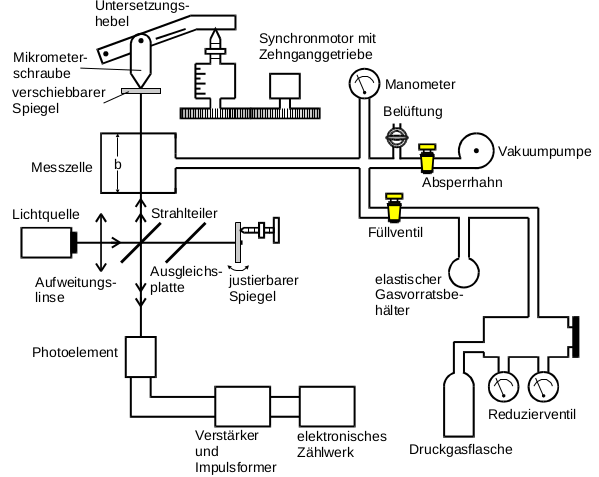
\includegraphics[scale=0.5]{aufbau.png}
  \caption{Aufbau der Messapparatur.}
  \label{fig:3}
\end{figure}
\subsection{Versuchsdurchführung}
\section{Auswertung}
\subsection{Wellenlänge eines Helium-Neon-Lasers}
\begin{table}[h]
  \centering
  \caption{Messwerte für die Messung an einem Helium-Neon-Laser sowie für jedes Wertepaar
  berechnete Wellenlänge.}
  \begin{tabular}{c c c}
    \toprule
    $\symup{\Delta}d$ / \si{\milli\metre} & $z$ & $\lambda$ \\
    \midrule
    2 & 1286 & 619.98 \\
    2 & 1327 & 600.82 \\
    2 & 1284 & 620.94 \\
    2 & 1305 & 610.95 \\
    2 & 1340 & 594.99 \\
    2 & 1288 & 619.01 \\
    2 & 1326 & 601.27 \\
    2 & 1300 & 613.30 \\
    2 & 1330 & 599.47 \\
    2 & 1292 & 617.10 \\
    \bottomrule
  \end{tabular}
  \label{tab:1}
\end{table}

Die Messwerte finden sich in Tabelle \ref{tab:1}. Ebenfalls in dieser Tabelle finden
sich die nach \eqref{eq:1} berechneten Wellenlängen. Die an der Millimeterschraube
gemessenen Verschiebungen müssen durch die Hebelübersetzung von \num{5.017} geteilt
werden, um die tatsächliche Verschiebung des Spiegels zu erhalten.
Durch Mittelwertbildung erhält man einen Wert von:
\begin{align*}
  \lambda = \SI{609.8(31)}{\nano\metre}.
\end{align*}

\subsection{Brechungsindex von Luft und CO2}

\begin{table}[h]
  \centering
  \caption{In Tabelle \subref{tab:2} sind die gemessenen Werte bei Füllung der
  Kammer mit Luft, in Tabelle \subref{tab:3} für CO2 eingetragen. Außerdem
  eingetragen ist der für jedes Wertepaar berechnete Brechungsindex $n$.}
  \label{tab:4}
    \begin{subtable}{0.49\textwidth}
    \centering
    \begin{tabular}{c c c}
      \toprule
      $P$ / \si{\bar} & $z$ & $n$ \\
      \midrule
      0.2132 & 46 & 1.000416 \\
      0.2132 & 33 & 1.000298 \\
      0.2132 & 47 & 1.000425 \\
      0.2132 & 32 & 1.000289 \\
      0.2132 & 37 & 1.000334 \\
      0.2132 & 35 & 1.000316 \\
      0.2132 & 33 & 1.000298 \\
      0.2132 & 50 & 1.000452 \\
      0.2132 & 34 & 1.000307 \\
      0.2132 & 33 & 1.000298 \\
      \bottomrule
    \end{tabular}
    \caption{Werte für Luft.}
    \label{tab:2}
  \end{subtable}
    \begin{subtable}{0.49\textwidth}
    \centering
    \begin{tabular}{c c c}
      \toprule
      $P$ / \si{\bar} & $z$ & $n$ \\
      \midrule
      0.2132 & 52 & 1.000470 \\
      0.2132 & 50 & 1.000452 \\
      0.2132 & 50 & 1.000452 \\
      0.2132 & 51 & 1.000461 \\
      0.2132 & 53 & 1.000479 \\
      0.2132 & 52 & 1.000470 \\
      0.2132 & 50 & 1.000452 \\
      0.2132 & 50 & 1.000452 \\
      0.2132 & 52 & 1.000470 \\
      0.2132 & 52 & 1.000470 \\
      \bottomrule
    \end{tabular}
    \caption{Werte für CO2.}
    \label{tab:3}
    \end{subtable}
\end{table}

Zur Bestimmung der Brechnungsindize der beiden Gase nach \eqref{eq:3} (mit \eqref{eq:2})
sind einige Werte notwendig. Diese sind wie folgt:
\begin{align*}
  \text{Normaldruck: } p_0 =& \; \SI{1.0132}{\bar} \\
  \text{Normaltemperatur: } T_0 =& \; \SI{273.15}{\kelvin} \\
  \text{Umgebungstemperatur: } T =& \; \SI{293.15}{\kelvin} \\
  \text{Durchmesser der Zelle: } b =& \; \SI{50}{\milli\metre} \\
  \text{Wellenlänge Laser: } \lambda =& \; \SI{635}{\nano\metre}. \\
\end{align*}
Weiter ist zu beachten, dass sich die Kammer in allen Fällen nur auf \SI{-0.8}{\bar}
evakuieren ließ, sodass der verbeleibende Kammerinnendruck bei \SI{0.2132}{\bar}
lag. Der Nullpunkt der Skala des Manometers ist auf $p_0$ geeicht. Die gemessenen
Werte sowie die nach \eqref{eq:3} bestimmten Brechungsindize sind in Tabelle \ref{tab:4}
dargestellt. Der in den Rechnungen benötigte Wert $\symup{\Delta}n$ wird nach \eqref{eq:2}
bestimmt. Aufgrund der großen Abweichung zwischen dem auf dem Laser angegebenen und dem
oben bestimmten Wert für $\lambda$ wird ersterer in den Rechnungen genutzt. Es ergeben
sich folgende Mittelwerte:
\begin{align*}
  n_\symup{Luft} =& \; \num{1.000343(20)} \\
  n_\symup{CO2} =& \; \num{1.000463(3)}. \\
\end{align*}

\section{Diskussion}
Im Vergleich mit dem auf dem Laser angebenen Wert von \SI{635}{\nano\metre} für die
Wellenlänge zeigen sich Abweichungen, die nicht im Bereich der Messungenauigkeiten liegen.
Es ist daher von einem systematischen Fehler auszugehen. Denkbar sind vorallem
Fehlzählungen. Auch wenn die Geschwindigkeit, mit der der Spiegel verstellt wurde,
extrem gering war, kann nicht ausgeschlossen werden, dass die Frequenz, mit der
die resultierenden Maxima am Photodetektor vorbeizogen das Auflösungsvermögen eben
dieses überstiegen.\\
Bei Vergleich zwischen den für die Brechungsindize gemessenen Werten mit Literaturwerten
von \num{1.0002765}\cite{luft} für Luft und \num{1.0004476}\cite{co2} für CO2 zeigen
sich ebenfalls keine Übereinstimmungen im Fehlerintervall. Die relativen Abweichungen
sind mit \num{4.65e-3} und \SI{1.24e-3}{\percent} jedoch extrem gering. Auch hier sind
Fehlzählungen das Wahrscheinlichste. Eine erneute Messung mit einem genaueren Messgerät
sollte daher alle Werte verbessern können.
\newpage
\nocite{*}
\printbibliography
